\chapter{Kalman Filters}
\label{Kalman Filters}

The Kalman Filter (KF) generates predictions for linear dynamical systems \cite{inbook}. Assuming the given data is noisy and Gaussian \cite{inproceedings, article7}, the first predictive step assumes knowledge of initial states and the model process. The next step involves calculating the covariance in order to calculate the Kalman Gain, which is a measure of how much the estimate should be changed given actual measurements of the system. The corrective step utilizes the Kalman Gain and the measured system outputs to gauge whether to depend more on the model or on the data. This process can be done recursively, allowing the model to become progressively more accurate as more data is added. Therefore, overtime, it is expected that the model will converge with the actual system measurements.
\\  \\
The Kalman Filter had many aeronautical applications, which include long-distance flight, autopilots, space exploration and military defense systems. In fact, was even used in the Apollo Program  \cite{kalmanbio}. 

\begin{figure}[h]
    \centering
    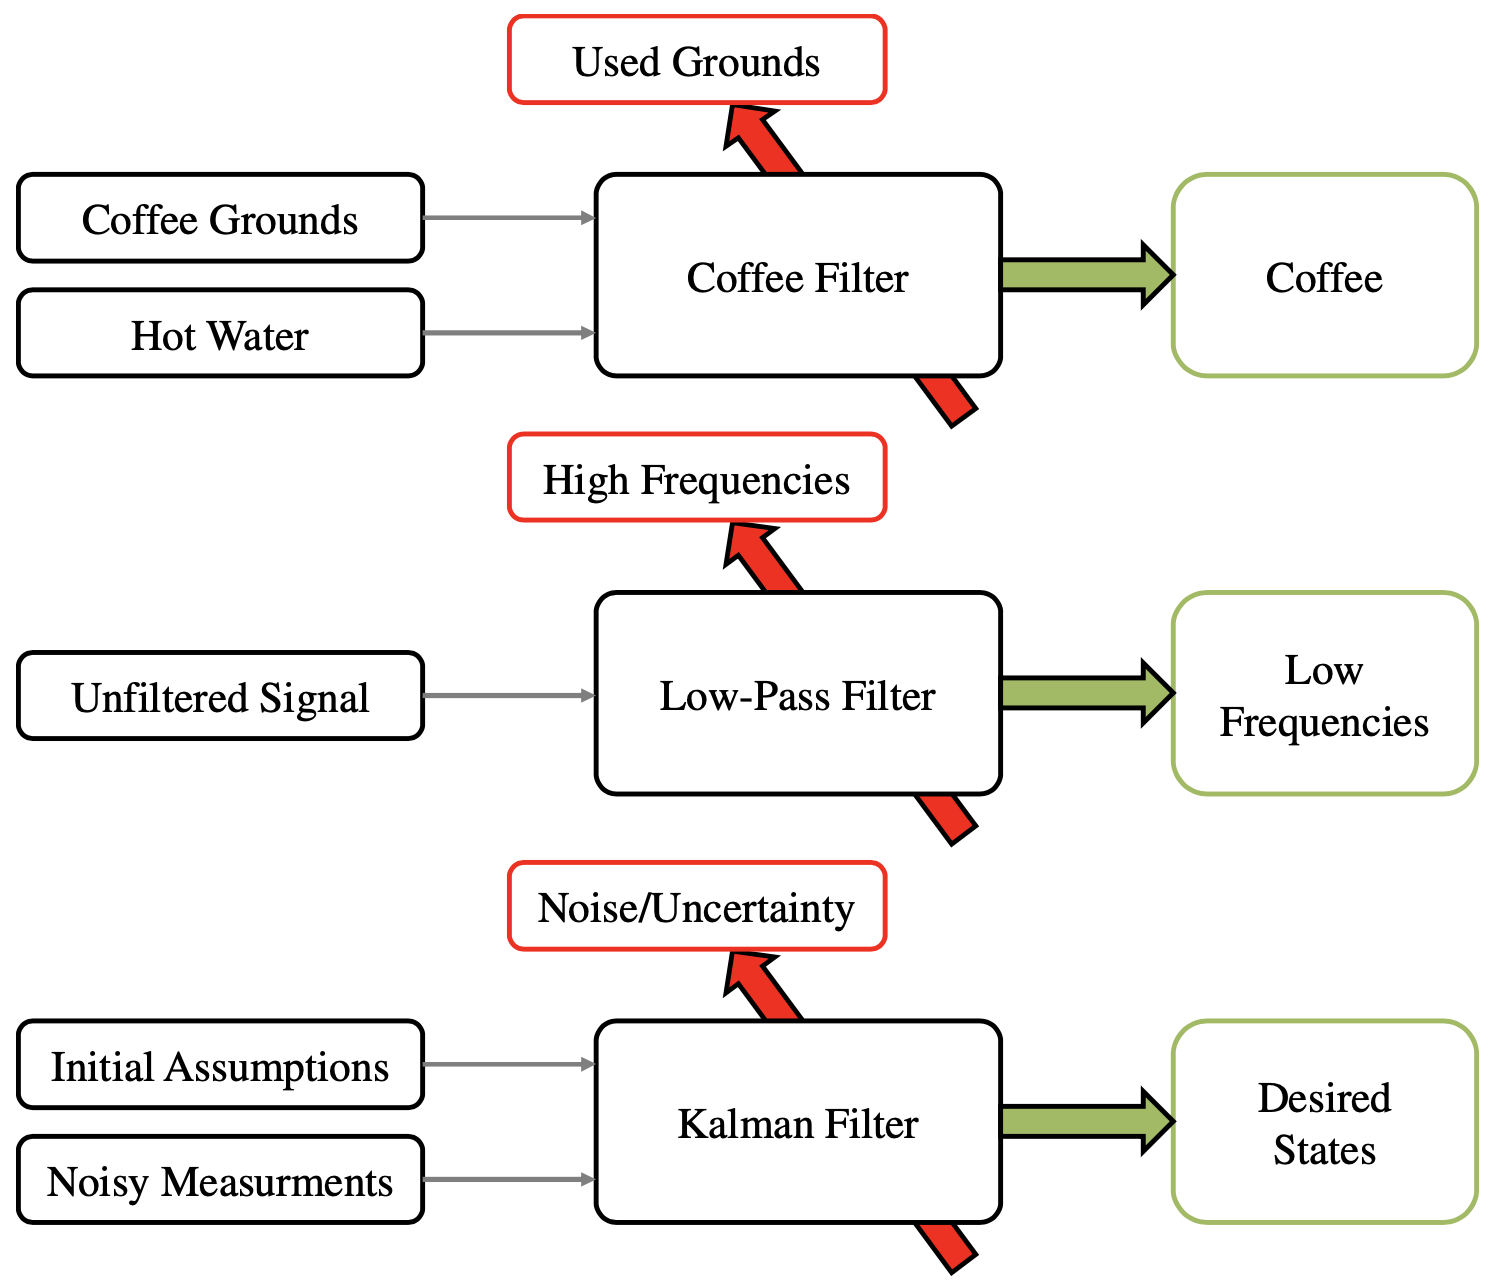
\includegraphics[scale = 0.4]{coffee.png}
    \caption{A screen-shot taken from a paper by Rhudy et al. comparing the Kalman Filter to a coffee filter \cite{article7}.}
    \label{coffee}
\end{figure}

\newpage

\begin{figure}[h]
    \centering
    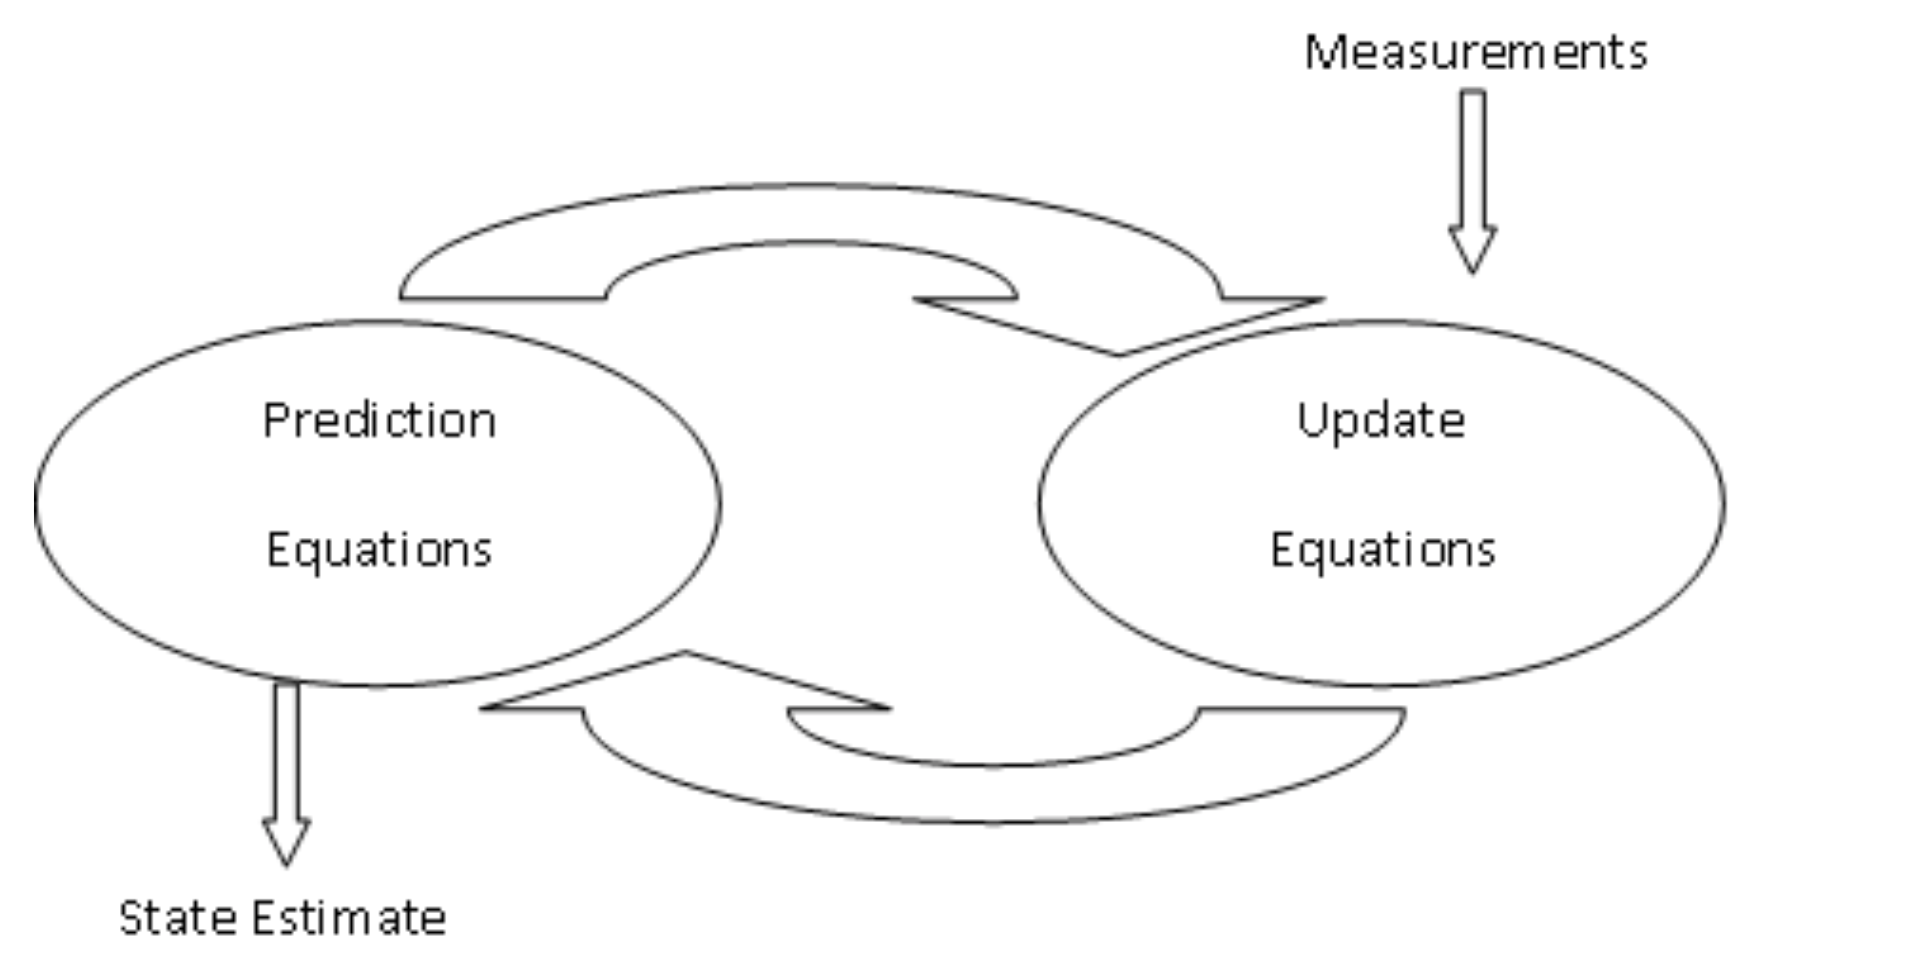
\includegraphics[scale = 0.3]{diagram.png}
    \caption{A basic diagram of the Kalman Filter \cite{kohanbash_2014}.}
    \label{coffee}
\end{figure}

\newpage

\noindent The Kalman Filter is named after its developer, Rudolph Emil Kalman. Kalman was born on May 19, 1930 in Budapest, Hungary. After arriving in the United States, Kalman completed his undergraduate studies and masters degree in electrical engineering from Massachusetts Institute of Technology  and completed his doctoral degree in Columbia University. He would spend the next years of his life teaching. In the 1960s to 1970s he became a professor at Stanford university \cite{kalmanbio}. In the 1970s and 1990s, Kalman spent time as professor of  engineering at the University of Florida. Kalman is most known for his work on the Kalman Filter, which was developed in the late 1950s. The Kalman Filter greatly aided the United States' military projects, resulting in formed President Obama to award Kalman the National Medal of Science in 2009. In addition, in 1985, Kalman was awarded the Kyoto Prize, which is the Japanese version of the Nobel Peace Prize in the united States. Kalman passed away July 2, 2016 at the age of 86 and is survived by his wife and two children \cite{Kalman_bio}. 


\newpage

\section{Kalman Filter Algorithm}

The Kalman Filter predicts the system's state variable at the next time step given knowledge of the system. This is modeled by the formula.  

\begin{align*}
       x_{k+1} = F x_k + w_k,
    \end{align*}
    where $x_{k+1}$ is the state system at the next time step, $F$ is the state function, and $w_k$ is process noise. Here, measurement noise is normally distributed with a mean of 0.

To initialize the model, it is assumed that the state system at step 0 is normally distributed, or
\begin{align*}
	x_0 = N(m_0, c_0),
\end{align*}
	where $m_0$ is the mean of the data and $c_0$ is the covariance.
The estimate of the the system measurement, $y_k$, is given by 
\begin{align*}
	y_k = H x_k + v_k,
\end{align*}
where $H_k$ is the observation function and $v_k$ is measurement noise, Here, $v_k$ is normally distributed with a mean of 0. The initial assumption, measurement noise, and process noise are all independent of one another.
	
	

\begin{enumerate}
  \item Begin by initializing the state estimate and the initial state covariance matrix. The state estimate, $x_0$, can be found by taking the expected value of the data where data is normally distributed. If the system states are finite, the expectation is denoted by
    \begin{align*}
        x_0 = \mathbb{E}[x_0]  = \begin{bmatrix}
           x_1 \\
           \vdots \\
           x_n 
         \end{bmatrix}.
      
    \end{align*}
    The state covariance matrix, $P_0$, is a square matrix whose contents are the covariance of the pairwise elements
    \footnote{Recall that the covariance of a variable with itself is the variance of the variable}
    , or
    \begin{align*}
      P_0 =
      \begin{bmatrix}
           var(x_1)  & \hdots & cov(x_1,x_n) \\
           \vdots & \ddots & \vdots \\
           cov(x_n, x_1)  & \hdots & var(x_n )
         \end{bmatrix} .
  \end{align*}
  Enough should be known about the modeled system to generate these values. In general, $\hat x_k$ denotes the model's estimate of the state variables. When initializing these values, we use $x_0$, which is the actual initial measurements of the system. \\ \\
   A state covariance matrix is a symmetrical positive semi-definite square matrix whose diagonals correspond to the variance of a variable at location i and elsewhere is the covariance of the pairwise elements. In practice, covariance matrices help us better understand the spread of data. For the case of the KF, calculating the state covariance is necessary for computing Kalman Gain. 
   
   
  \item After initializing the state estimate and state covariance, a prediction can be generated. The estimate of the system at the next time step, $x_{k+1}$,  is given by
  \begin{align*}
      x_{k+1} = F x_{k} +  G u_{k} + w_{k} ,
  \end{align*} 
  where $F$ is the state matrix, $G$ is the F and input matrix, $u_k$ is an input vector and $w_k$ is the process noise vector. Every state variable contained in $x_k$ is defined by a linear differential equation. These linear differential equations can be used to generate the F and G matrices. Therefore, F should be a square matrix whose dimension is equal to the number of states variables and G can be a matrix (or in some cases a vector), depending on the dimension of input vector u. \\ \\
  $u_k$  is an input vector, which is a measurable value that helps define the system, but is not contained in the state vector. Depending on how the system is defined, $u_k$  can be a constant value or it can be a value dependent on time step k. \\ \\
  $w_k$ is the process noise vector at time k. Process noise can be thought of as the model's accuracy. When process noise is 0, it implies that the model is perfectly accurate and does not have to correct for incoming system measurements. On the other hand, high process noise will essentially restate the system based on incoming measurements. $w_k$ has the same dimensions as $x_k$, allowing us to identify whether or not to adjust the equations for the state variables. When all values of  $w_k$ equal 0, it implies that the linear differential equations we are using to define the state variables have no error. 
  
  
  
  \item Next, the state covariance matrix to calculate Kalman Gain. The state covariance matrix at time step $k$ given the last time step, is 
    \begin{align*} 
        P_{k | k -1} = F P_{k - 1} F^T + Q_{k-1}, 
    \end{align*}
    where $F^T$ is the transpose of $F$, and $Q_{k}$ is the process noise covariance of $w_k$.
    The Kalman Gain at time step $k$, is given by
    \begin{align*} 
        K_k = P_{k | k - 1} H^T_K (H_k P_{k | k - 1} H^T_K + R_k)^{-1},
    \end{align*}
      where $H$ is the observation matrix and $R$ is measurement noise covariance. 
      $H$ enables the state variables to be linearly transformed to match the outputs of the system. The dimensions of $H$ reflects which state variables have measurable values in the system. It is not assumed that every state variable is measurable, so $H$ allows us to compare the measurable state variables to $x_k$. Simple applications of $H$ include creating matrices with 0's and 1's, with 1's denoting that a state variable is measurable and a 0's representing non-measurable states. In other cases, $H$ is an integer used as a scaling factor. \\ \\
     The Kalman Gain is the main component of the corrective aspect of the KF. The Kalman Gain is a measure of how much to change the model based on incoming data. Low values of the Kalman Gain imply the model is accurate while higher values indicate the model should adjust based on the incoming data.  \\ \\
     From this equation, one can see that balancing $Q$ and $R$ is critical for model performance. Larger values of $Q$ indicate higher modeling error, which leads to a higher Kalman Gain and increased model correction. On the other hand, large values of $R$ imply high measurement error, leading to a lower Kalman Gain and less model correction. 
     
   
    \item Next, calculate the transformed output vector and correct the prediction. The transformed output vector, $\hat y_k$, is given by
    \begin{align*}
        \hat y_k = H_k x_k + v_k,
    \end{align*}
    
    where $v_k$ is measurement noise, which is added to account for measurement error.
    The corrected prediction, $x_k$, is given by:
    \begin{align*} 
        x_k = x_{k - 1} + K_k(y_k - \hat y_{k}),
    \end{align*}
   where  $y_k$ is the actual measurements of the system, $K_k$ is the Kalman Gain, and $x_{k-1}$ are the values of the state variable at the last time step. $\hat y_k$ is a way of transforming the prediction (using $H$) into a format that can be compared with $y_k$. Subtracting the actual measurements from the predicted measurements is necessary, because $y_k$ does not always contain measurements for all variables in state vector $x_k$. The quantity $y_k - \hat y_{k}$ is also known as measurement residual or innovation.  \\
   
     \item The final step is to update the state covariance matrix, $P_k $, through the equation:
    \begin{align*} 
        P_k = (I - K_k H_k) P_{k | k-1},
    \end{align*}
    where $I$ is the identity matrix, $K_k$ is the Kalman Gain, $H_k$ is the obersevation function, and $P_{k|k-1}$ is the state covariance at time step $k$ given the last time step. $ P_k $ will be used in the next iteration of the filter.
\end{enumerate} 


\newpage

\begin{center}
\begin{table}
\centering
\caption{Description of all variables in the Kalman Filter} \label{tab:sometab}
\begin{tabular}{ |p{2cm}||p{5cm}|p{2cm}| }
    \hline
    \multicolumn{3}{|c|}{Variables in the Kalman Filter } \\ 
    \hline
    Variable & Description & Dimensions \\
    \hline
    x & State variables  & $d_x \times 1$ \\
    y & Output vector  & $d_y \times 1$ \\
    u & System inputs  & $d_u \times 1$\\
    v & Measurement noise & $d_y \times 1$\\
    w & Process noise & $d_x \times 1$\\
    F & State function  & $d_x \times d_x $  \\ 
    H & Observation function & $d_y \times d_x$\\
    G & Input function & $d_x \times d_u$\\
    K & Kalman Gain  & $d_x \times d_y$\\
    Q & Process noise covariance  & $d_x \times d_x$ \\
    R & Measurement noise covariance &  $d_y \times d_y$\\
    P & Covariance matrix & $d_x \times d_x $  \\ 
    
    \hline
\end{tabular}

\end{table}
\end{center} 




